% !TeX root = ../paper.tex
% !TeX encoding = UTF-8
% !TeX spellcheck = en_US

\section{Evaluation}\label{sec:evaluation}

  In this section, we present an initial evaluation of the performance and fault-tolerance of our algorithm.
  In \cref{sec:evaluation:correctness}, we evaluate the correctness of the results produces by our algorithm when run in different settings and under faults, \cref{sec:evaluation:comparison} then compares the performance with our baseline \ocddiscover{} by \citeauthor{consonni}.
  \Cref{sec:evaluation:scalability} then explores further the scalability of \dodo{} across multiple nodes.
  The code for \ocddiscover{} was provided to us by the authors.

  To evaluate the performance of the different \gls{od} discovery approaches, we measure the overall runtime of the algorithm needed to compute all \glspl{od} and \glspl{ocd}.
  The runtime of the algorithm includes startup and shutdown times and the algorithm must terminate to produce a valid result.
  As a consequence, when running \dodo{} in a distributed setting, this measurement will include node discovery and shutdown synchronization times.

  All experiments were performed on homogeneous nodes with 20 cores and 64~GB of main memory.
  \dodo{} is implemented in Scala and the nodes run it with Java 1.8 with the Java JVM heap space limited to 40~GB.
  We adopted the \textit{flight\_1k} dataset available from the Information Systems Group at Hasso Plattner Institute\footnote{\url{https://hpi.de/naumann/projects/repeatability/data-profiling/fds.html}} to reduce the computation time to an order of minutes.
  This was achieved by removing sparse columns%
  \footnote{Removed columns: ArrivalDelayGroups, CancellationCode, Cancelled, CarrierDelay, CRSArrTime, DepartureDelayGroups, DepTimeBlk, Dest, DestAirportID, DestAirportSeqID, DestCityMarketID, DestCityName, DestState, DestStateFips, DestStateName, DestWac, DistanceGroup, Div1Airport, Div1AirportID, Div1AirportSeqID, Div1LongestGTime, Div1TailNum, Div1TotalGTime, Div1WheelsOff, Div1WheelsOn, Div2Airport, Div2AirportID, Div2AirportSeqID, Div2LongestGTime, Div2TailNum, Div2TotalGTime, Div2WheelsOff, Div2WheelsOn, Div3Airport, Div3AirportID, Div3AirportSeqID, Div3LongestGTime, Div3TailNum, Div3TotalGTime, Div3WheelsOff, Div3WheelsOn, Div4Airport, Div4AirportID, Div4AirportSeqID, Div4LongestGTime, Div4TailNum, Div4TotalGTime, Div4WheelsOff, Div4WheelsOn, Div5Airport, Div5AirportID, Div5AirportSeqID, Div5LongestGTime, Div5TailNum, Div5TotalGTime, Div5WheelsOff, Div5WheelsOn, DivActualElapsedTime, DivAirportLandings, DivArrDelay, DivDistance, DivReachedDest, FirstDepTime, LateAircraftDelay, LongestAddGTime, NASDelay, SecurityDelay, TaxiIn, TaxiOut, TotalAddGTime, WeatherDelay, WheelsOff, WheelsOn}.
  We ended up with a dataset consisting of 1000 rows and 36 columns: \textit{flight\_r1k\_c36}.

\subsection{Correctness and fault-tolerance}\label{sec:evaluation:correctness}

  Because we based our approach on \ocddiscover{} by \citeauthor{consonni}, we don't expect our algorithm to output a complete minimal set of \glspl{od}.
  Our goal is to output the same \glspl{ocd} and \glspl{od} than \ocddiscover{}.

  We find that for all four datasets, which we considered for comparing the results, \dodo{} computes the same \glspl{ocd} and \glspl{od} independent of whether \dodo{} is running on a single node or distributed across multiple nodes.
  We did not compare the actual results for our medium-size test dataset \textit{flight\_r1k\_c36}, because it contains too many \glspl{od}.
  But \cref{tab:results} shows, that \dodo{} finds the same number of \glspl{od} in the dataset as \ocddiscover{}.
  The number of found \glspl{od} in \cref{tab:results} indicates the sum of found \glspl{ocd} and \glspl{od}.
  \texttt{iw,jn, kfailure(s)} indicates an experiment with \dodo{} using \texttt{i} workers per node, the system consisting of \texttt{j} nodes overall and \texttt{k} nodes of them were killed during the experiment.

  \begin{table}
    \centering
    \begin{tabular}{lrrrr}
      \toprule
      \textbf{Experiment} & \textbf{CCs} & \textbf{OECs} & \textbf{\glspl{od}} & \textbf{runtime} \\
      \midrule
      \texttt{\ocddiscover{}, 8w} & 7 & 5 & 49~514 & 7~m~09~s \\
      \texttt{8w, 1n, 0failure} & 7 & 5 & 49~514 & 3~m~42~s \\
      \texttt{8w, 8n, 0failure} & 7 & 5 & 49~514 & 49~s \\
      \texttt{8w, 8n, 1failure} & 7 & 5 & 50~055 & 54~s \\
      \texttt{8w, 8n, 2failures} & 7 & 5 & 48~374 & 55~s \\
      \texttt{8w, 8n, 3failures} & 7 & 5 & 48~352 & 52~s \\
      \bottomrule
    \end{tabular}
    \caption{Result comparison between \ocddiscover{}, \dodo{}, and \dodo{} in the presence of node failures.}
    \label{tab:results}
  \end{table}

  If \dodo{} experiences node failures, it redistributes the \gls{od} candidates to the remaining nodes using the state replication protocol (see \cref{protocol:stateReplication}).
  This leads to duplicate checks and along with that to the same \gls{od} being found multiple times.
  This is the case in the experiment \texttt{8w, 8n, 1failure}.
  \dodo{} finds more \glspl{od} in this experiment as there are in the dataset.
  This is due to the fact that we do not yet perform deduplication of the found \glspl{od}.

  The experiments with two and more failing nodes do not find all \glspl{od} in the dataset.
  Unfortunately, we performed the experiments manually and the first node failure was introduced before the node was able to replicate its state to the other nodes in the cluster.
  This caused the system to loose all \gls{od} candidates of this node.
  But \dodo{} was able to recover from the following node failures, because those nodes were already able to replicate their state.

  In \cref{tab:results}, we already notice that \dodo{} in a single nodes setup with eight workers is nearly 2x as fast as \ocddiscover{} with eight threads.
  Running \dodo{} on multiple nodes decreases the time even more as one would expect.
  If there are no failures, \dodo{} outputs the correct results independent of the number of nodes it is deployed on.
  
\subsection{Comparing with \ocddiscover{}}\label{sec:evaluation:comparison}

  In \cref{fig:runtime-vs-ocddiscover}, we compare the performance of \dodo{} with \ocddiscover{} on a single node using our test dataset.
  \ocddiscover{} is only capable of running on a single-node setup, but can scale by increasing the number of used threads.
  We measure the runtime of the algorithms to find all \glspl{od} with a different degree of parallelism.
  \ocddiscover{} scales by increasing the number of threads and \dodo{} scales with the number of workers in a single node setup.

  \begin{figure}
    \centering
%    \includestandalone{pictures/tikz/runtime-vs-ocddiscover}
    % !TeX root = ../../paper.tex
% !TeX encoding = UTF-8
% !TeX spellcheck = en_US

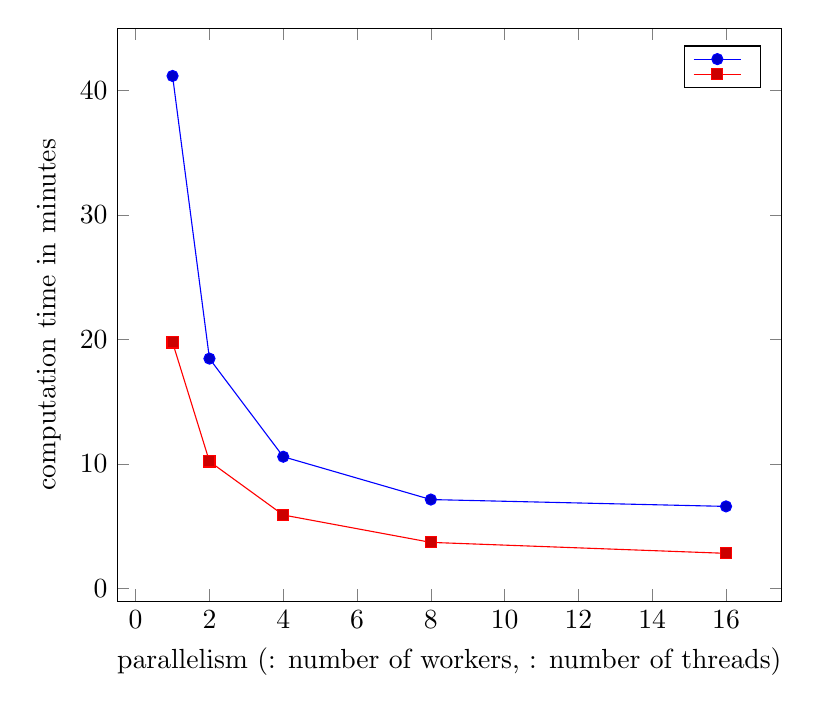
\begin{tikzpicture}
  \begin{axis}[
    scale only axis,
    xlabel={parallelism (\dodo{}: number of workers, \ocddiscover{}: number of threads)},
    ylabel=computation time in minutes,
    legend pos=north east,
    legend cell align={left},
  ]

    \addplot coordinates {
      (1, 41.17)
      (2, 18.47)
      (4, 10.59)
      %      (6, 0.00)
      (8, 7.15)
      %      (10, 0.00)
      %      (12, 0.00)
      %      (14, 0.00)
      (16, 6.60)
    };

    \addplot coordinates {
      (1, 19.77)
      (2, 10.21)
      (4, 5.91)
      %      (6, 4.41)
      (8, 3.71)
      %      (10, 2.98)
      %      (12, 2.98)
      %      (14, 2.92)
      (16, 2.83)
    };

    \legend{\ocddiscover{}, \dodo{}}

  \end{axis}
\end{tikzpicture}
    \caption{Single node runtime comparison of our approach and the baseline algorithm \ocddiscover{} with the test dataset \textit{flight\_1k\_stripped\_columns.csv}.}
    \label{fig:runtime-vs-ocddiscover}
  \end{figure}

  We find that \dodo{} with a single worker already outperforms the single-threaded version of \ocddiscover{} by over a factor of two.
  \ocddiscover{} switches to a completely different implementation when it is run multi-threaded.
  This version performs slightly better compared to \dodo{}, because \dodo{} can only achieve a performance increase by a factor of around 1.8.
  But besides that, \dodo{} scales better than \ocddiscover{}.
  \dodo{} achieves a performance increase of a factor of 2.8 when run with 18 workers compared to \ocddiscover{} with 18 threads.
  This shows that our implementation using the actor model with no explicit synchronization barriers is superior to the explicit multi-threading implementation by \citeauthor{consonni}.

\subsection{Scalability}\label{sec:evaluation:scalability}

  In \cref{sec:evaluation:comparison}, we already showed that \dodo{} outperforms our baseline \ocddiscover{} in a single node setup.
  In this section, we analyze the scalability of \dodo{} when run on multiple nodes in a cluster setup.

  \Cref{fig:node-scaling} shows the results of our cluster scalability experiments using our test dataset \textit{flight\_1k\_stripped\_columns.csv}, where we measured the runtime of \dodo{} with different cluster sizes.
  \Cref{fig:fig:node-scaling} plots the speed of running \dodo{} on multiple nodes and \cref{fig:tab:node-scaling} shows the actual runtime of \dodo{}.

  \begin{figure}[htbp]
    \centering
    \begin{subfigure}[c]{0.6\textwidth}
      \centering
      % !TeX root = ../../paper.tex
% !TeX encoding = UTF-8
% !TeX spellcheck = en_US

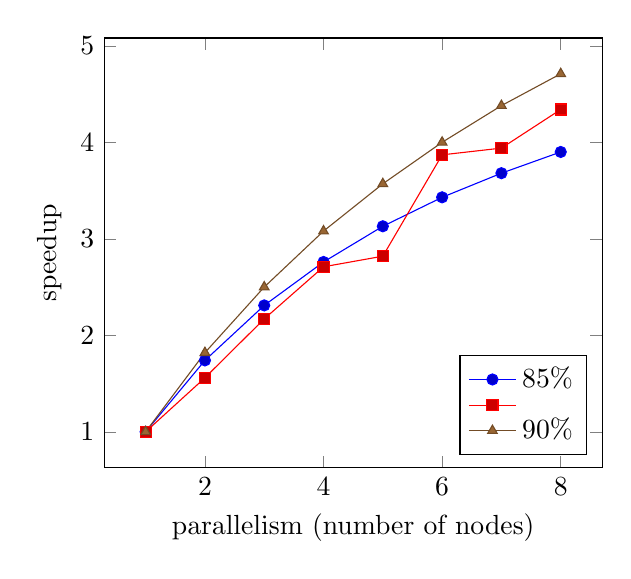
\begin{tikzpicture}[baseline=(current bounding box.center)]
  \begin{axis}[
    scale only axis,
    scale=0.75,
    xlabel=parallelism (number of nodes),
    ylabel=speedup,
    legend pos=south east,
    legend cell align={left},
  ]

    \addplot coordinates {
      (1, 1.00)
      (2, 1.74)
      (3, 2.31)
      (4, 2.76)
      (5, 3.13)
      (6, 3.43)
      (7, 3.68)
      (8, 3.90)
    };

    \addplot coordinates {
      (1, 1.00)
      (2, 1.56)
      (3, 2.17)
      (4, 2.71)
      (5, 2.82)
      (6, 3.87)
      (7, 3.94)
      (8, 4.34)
    };

    \addplot+[mark=triangle*] coordinates {
      (1, 1.00)
      (2, 1.82)
      (3, 2.50)
      (4, 3.08)
      (5, 3.57)
      (6, 4.00)
      (7, 4.38)
      (8, 4.71)
    };

    \legend{{$85 \%$},\dodo{},{$90 \%$}}
  
  \end{axis}
\end{tikzpicture}
      \caption{Computation time speedup of \dodo{} compared to theoretical $85 \%$ and $90 \%$ speedup.}
      \label{fig:fig:node-scaling}
    \end{subfigure}
    \begin{subtable}[c]{0.39\textwidth}
      \centering
      \begin{tabular}{cr}
        \toprule
        \textbf{\# nodes} & \textbf{computation time} \\
        \midrule
        1 & 3~m~37~s \\
        2 & 2~m~19~s \\
        3 & 1~m~40~s \\
        4 & 1~m~20~s \\
        5 & 1~m~17~s \\
        6 & 56~s \\
        7 & 55~s \\
        8 & 50~s \\
        \bottomrule
      \end{tabular}
      \caption{Computation time for finding all \glspl{od} in the dataset of different cluster sizes.}
      \label{fig:tab:node-scaling}
    \end{subtable}
    \caption{Scaling our algorithm over the number of nodes and keeping the number of workers fixed at eight workers per node using the test dataset \textit{flight\_1k\_stripped\_columns.csv}.}
    \label{fig:node-scaling}
  \end{figure}

  We find that using \dodo{} in a cluster setup greatly reduces overall computation time despite that additional effort is spend on node discovery, state replication and inter-node synchronization.
  Finding all \glspl{od} in our test dataset takes about three and a half minutes on a single nodes.
  This time is already reduced to under a minute when using six or more nodes in the \dodo{} cluster.
  As we can see in \cref{fig:fig:node-scaling}, \dodo{} can achieve a speedup between $85 \%$ and $90 \%$.
  The outliers in the diagram can be explained by our downing protocol implementation, which waits for all nodes to come to a mutual decision that all candidates were processed before shutting down nodes.
  This protocol can delay the shutdown procedure in unfortunate situations.
